\documentclass[presentation]{beamer}
\usepackage{common}
\usepackage{arydshln}

\newcommand{\cscat}[1]{$\langle\text{{\itshape#1}}\rangle$}
\newcommand{\csopt}[1]{{\itshape[}#1{\itshape]}}
\newcommand{\csalt}[1]{{\itshape(#1)}}
\newcommand{\op}[1]{\alert{`\texttt{#1}'}}
\newcommand{\operand}[1][\ldots]{{\normalcolor#1}}
\newcommand{\literal}[1]{\texttt{\alert{#1}}}
\newcommand{\bs}{$\backslash$}
\newcommand{\codepath}[1]{../../code/lecture-06/#1}

\AtBeginSubsection[]
{
  \begin{frame}<beamer>
    \frametitle{Next In Line\ldots}
    \tableofcontents[currentsection,currentsubsection]
  \end{frame}
}

\title[\lecturecode{06a}]{06a \\ \dotnet Exceptions}

\author[Giovanni Ciatto]{Giovanni Ciatto\\\texttt{giovanni.ciatto@unibo.it}}

\begin{document}

\frame[label=coverpage]{\titlepage}

\section{Overview}

\subsection{Compile-time vs. Run-time Errors}

\begin{frame}[allowframebreaks]{Compile-time vs. Run-time Errors}
  \bl{Compile-time Errors}{\iz{
    \item more common ones, can be detected by the \alert{compiler}
    \item they are part of the \alert{implementation phase} and provoke no harm
    \item as, in \alert{strongly-typed} languages, they commonly \alert{prevent compilation}
    \item modern editors and \alert{IDE} can reveal them during \alert{editing}
  }}

  \bl{Run-time errors ($\leftarrow$ object of this lesson)}{\iz{
    \item \alert{anomalous} situation that may occur as part of a system \alert{dynamics}  {\iz{
      \item[eg] unexpected parameters in method invocations, wrong ordering of method call, etc.
    }}
    \item it is commonly possible to \en{
      \item \alert{describe where} they may occur,
      \item \alert{intercept} them,
      \item \alert{handle} them via some compensation procedure
    }
    \item most OOP languages (e.g. Java or \csharp, unlike C) provide \alert{high-level constructs} to do so, namely \alert{exceptions}
  }}
\end{frame}

\begin{frame}{Run-time Errors, a.k.a. Exceptions}
  \begin{exampleblock}{About Exceptions}
    Exceptions are the way run-time errors are represented in modern OOP
    %
    \begin{itemize}
      \item they can be raised/thrown to signal an anomaly
      \item they can be catched to handle the anomaly
      \item when not catched they break/interrupt the execution of the program
    \end{itemize}
  \end{exampleblock}

  \begin{alertblock}{The Importance of Interrupting Anomalous Programs}
    \begin{itemize}
      \item Unexpected anomalies \alert{should} break the program \alert{as soon as possible}
      \item \ldots unlike segmentation faults in C
      \item to prevent the program from acting inconsistently or unexpectedly
    \end{itemize}
  \end{alertblock}
\end{frame}

\subsection{Common Exceptions}

\begin{frame}[allowframebreaks]{You May Have Already Met Some Exceptions}
  \tcodeview{3}{12}{14}{\tiny}{\codepath{Snippets/Program.cs}}{Division by zero}
  \tcodeview{3}{16}{18}{\tiny}{\codepath{Snippets/Program.cs}}{Stack overflow}
  \tcodeview{3}{20}{22}{\tiny}{\codepath{Snippets/Program.cs}}{Null reference}
  \framebreak
  \tcodeview{3}{24}{24}{\tiny}{\codepath{Snippets/Program.cs}}{Wrong format}
  \tcodeview{3}{26}{28}{\tiny}{\codepath{Snippets/Program.cs}}{Index out of range}
  \tcodeview{3}{30}{31}{\tiny}{\codepath{Snippets/Program.cs}}{Illegal Cast}
  assuming the following class hierarchy:
  \codeview{2}{34}{36}{\tiny}{\codepath{Snippets/Program.cs}}
\end{frame}

\subsection{\dotnet{} Exceptions}

\begin{frame}{\dotnet{} Exceptions}
  \begin{block}{Exceptions as types}
    \begin{itemize}
      \item \dotnet{} exceptions are \emph{reference} \alert{types}
      %
      \begin{itemize}
        \item in particular, they are sub-classes of \alert{\texttt{System.Exception}}
      \end{itemize}

      \item whose \alert{instances} can be \alert{thrown} to denote
      %
      \begin{itemize}
        \item an illegal operation/input/state---situation, in general
        \item an unexpected value
        \item some invariant of a class being violated
        \item an exceptional result
      \end{itemize}
    \end{itemize}
  \end{block}

  \begin{block}{Exception-related activities and \textbf{who} performs them}
    \begin{description}
      \item[throw] | performed by libraries \emph{implementors}
      \item[catch] | performed by libraries \emph{users}
      \item[design] | (rarely) performed by libraries \emph{designers}
      %
      \begin{itemize}
        \item[!] \dotnet class library is full of re-usable exceptions
      \end{itemize} 
    \end{description}
  \end{block}
\end{frame}

\begin{frame}{\dotnet{} Exceptions -- Example 1}
  \tcodeview{2}{7}{20}{\tiny}{\codepath{Snippets/MathUtils.cs}}{Exceptions as exceptional results}
  \codeview{3}{24}{25}{\tiny}{\codepath{Snippets/MathUtils.cs}}
\end{frame}

\begin{frame}{\dotnet{} Exceptions -- Example 2}
  \tcodeview{1}{5}{19}{\tiny}{\codepath{Snippets/Person.cs}}{Exceptions as violated invariants}
  \codeview{3}{25}{27}{\tiny}{\codepath{Snippets/Person.cs}}
\end{frame}

\begin{frame}{\dotnet Exception Type Hierarchy (non-exaustive)}
  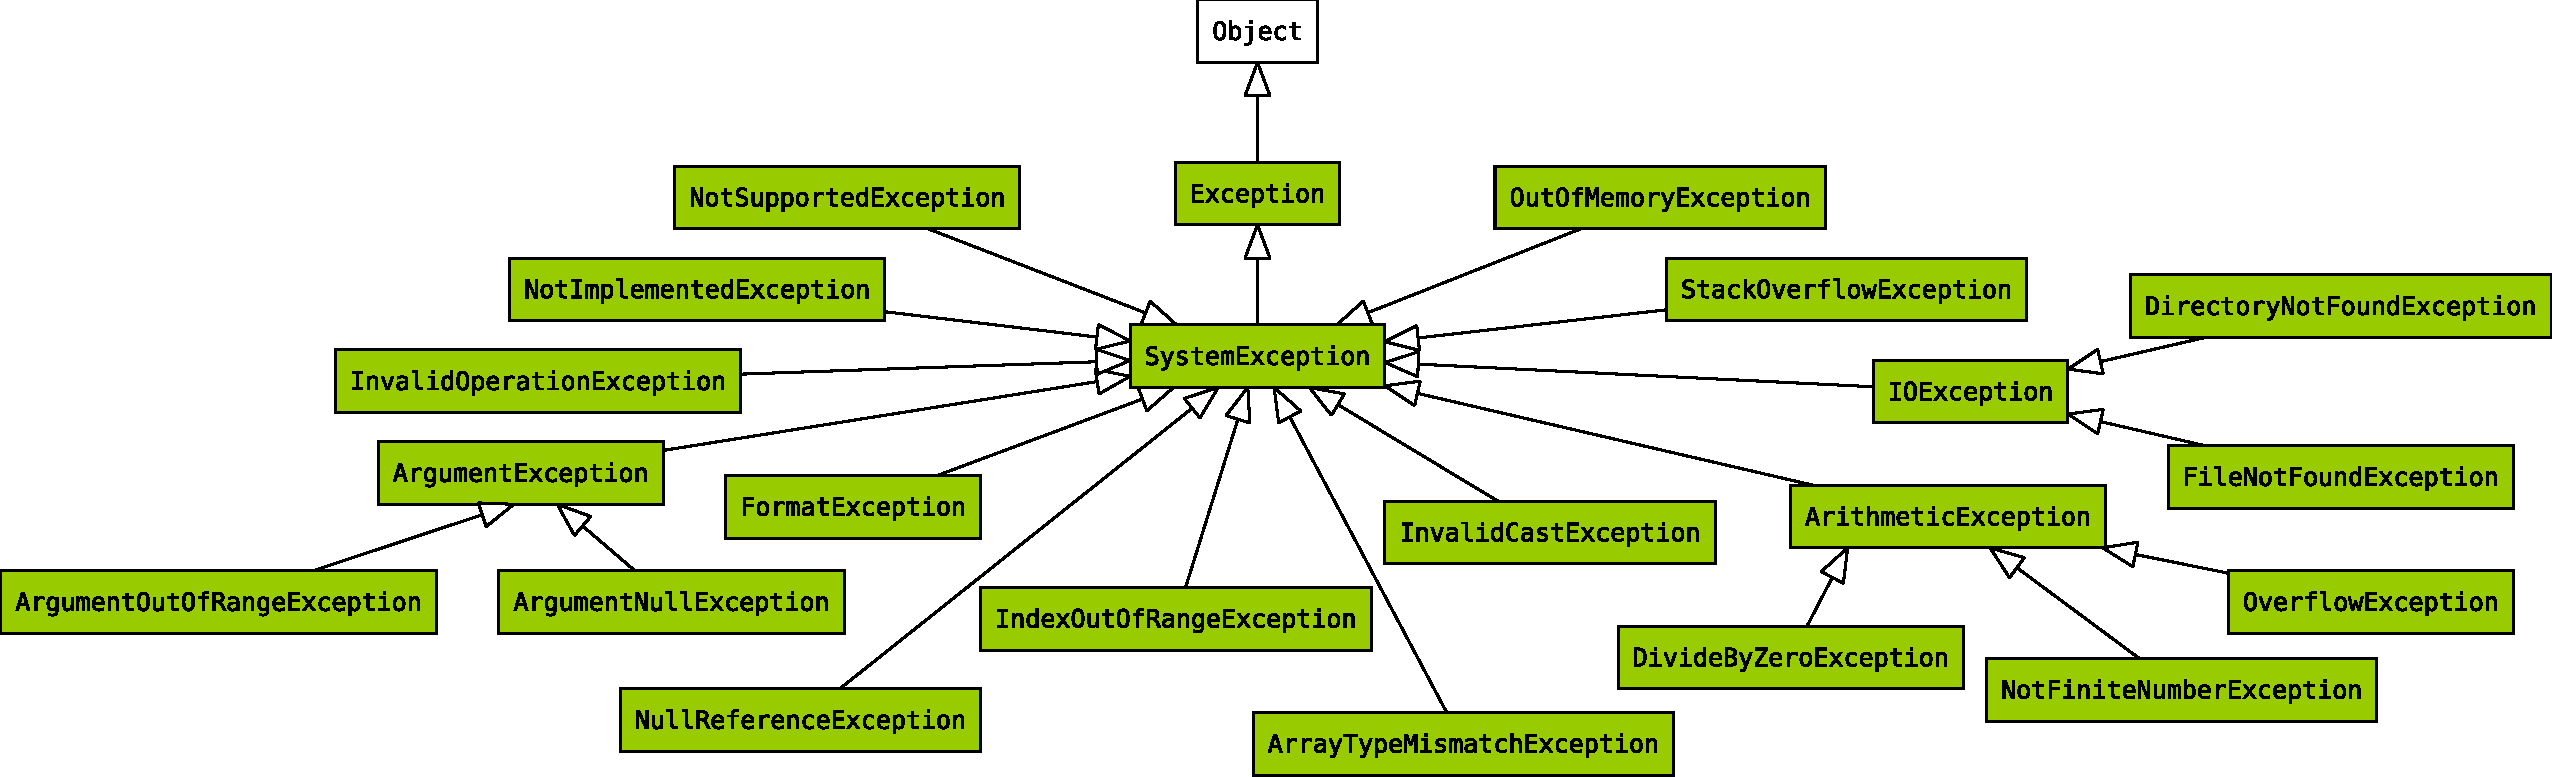
\includegraphics[width=\linewidth]{img/exception-hierarchy.pdf}
  %
  \begin{block}{Remarks}
    \begin{itemize}
      \item Notice the pivotal role of \alert{\texttt{SystemException}}
      %
      \begin{itemize}
        \item it is the base type of most common \emph{built-in} exceptions
        \item you may have met some of its subtypes :)
      \end{itemize}

      \item can you guess the \alert{naming} convention for exceptions?
      
      \item can you guess the \alert{purpose} of some of them?
    \end{itemize}
  \end{block}
\end{frame}

\begin{frame}[allowframebreaks]{Common Built-in Exceptions}
  \begin{description}
    \item[\texttt{NullReferenceException}] denotes an attempt to access some member of a \texttt{null} reference
    \smallskip 
    \item[\texttt{IndexOutOfRangeExecption}] denotes an attempt to access an index which is out of range (e.g. in arrays)
    \smallskip 
    \item[\texttt{ArrayTypeMismatchException}] denotes an attempt to insert an item of a wrong type into an array
    \smallskip 
    \item[\texttt{InvalidCastException}] denotes an attempt to perform some invalid cast/conversion
    \smallskip 
    \item[\texttt{InvalidOperationException}] a method call is invalid for the object's current state
    \smallskip 
    \item[\texttt{ArgumentException}] let method callers know that some argument they passed is wrong
    %
    \begin{description}
      \item[\texttt{ArgumentNullException}] an argument is unexpectly null
      \item[\texttt{ArgumentOutOfRangeException}] an argument is unexpectly out of some range (of some other argument) 
    \end{description}
    \smallskip
    \item[\texttt{ArithmeticException}] denotes some problem in computing some arithmetical operation
    %
    \begin{description}
      \item[\texttt{DivideByZeroException}] denotes an attempt to perform a division by zero
    \end{description}
    \smallskip
    \item[\texttt{IOExecption}] denotes some problem while performing some input/output operation
    \smallskip 
    \item[\texttt{NotSupportedException}] denotes that a functionality is (currently?) not supported
    \smallskip 
    \item[\texttt{NotImplementedException}] denotes that a functionality is (currently?) not implemented 
     %
     \begin{itemize}
      \item[!] commonly used as a \alert{placeholder} of functionalities to be implemented in stubs
    \end{itemize}  
    \framebreak  
    \item[\texttt{OutMemoryException}] there is no more memory to continue the execution of the program
    %
    \begin{itemize}
      \item[!] commonly happens when the heap is over, which may mean there's a \alert{memory leak}
    \end{itemize} 
    \smallskip 
    \item[\texttt{StackOverflow}] there is no more room on the stack to continue the execution of the program
    %
    \begin{itemize}
      \item[!] commonly happens when too many (recursive?) \alert{nested} method calls are performed
    \end{itemize}
  \end{description}
\end{frame}

\section{Throwing Exceptions}

\begin{frame}{The \texttt{throw} Statement}
  \begin{block}{Throw Statement}
    \begin{center}\ttfamily
        throw \cscat{Expression};
    \end{center}
    %
    \begin{itemize}
        \item where \texttt{\cscat{Expression}} returns a some instance of \texttt{Exception}:
        \item and it is usually something of the form:
        %
        \begin{center}\ttfamily\scriptsize
            new \cscat{Exception Type Name}(\cscat{Message})
        \end{center}
        %
        \begin{itemize}
          \item where \texttt{\cscat{Message}} is a string describing the issue which caused the exception
        \end{itemize}
    \end{itemize}
  \end{block}

  \codeview{3}{9}{9}{\tiny}{\codepath{Snippets/ThrowingExceptions.cs}}
  \codeview{3}{14}{16}{\tiny}{\codepath{Snippets/ThrowingExceptions.cs}}
  \codeview{3}{21}{23}{\tiny}{\codepath{Snippets/ThrowingExceptions.cs}}
\end{frame}

\begin{frame}[allowframebreaks]{What happens when an Exception is Thrown?}
  \begin{enumerate}
    \item The control flow is \alert{interrupted}
    
    \bigskip

    \item The control flow is given to any method in the current \alert{call stack} which is capable of \alert{catching} current exception
    
    \bigskip

    \item If none is found, \alert{the program execution is interrupted}\ldots
    
    \bigskip

    \item \ldots and the exception's \alert{stack trace} is shown.
    %
    \begin{itemize}
      \item to let programmers \alert{locate} the issue in the code
    \end{itemize}
  \end{enumerate}

  \framebreak

  Consider for instance the following method:
  %
  \codeview{2}{26}{37}{\tiny}{\codepath{Snippets/ThrowingExceptions.cs}}  
  %
  and suppose it is invoked like this:
  %
  \codeview{3}{41}{41}{\tiny}{\codepath{Snippets/ThrowingExceptions.cs}}  
  %
  then, the following \alert{stack trace} is printed
  %
  \lstinputlisting[language={},basicstyle=\tiny\ttfamily]{./snippets/StackTrace.txt}
  %
  whereas the many \texttt{Console.WriteLine(\ldots)} are \alert{not} executed.

\end{frame}

\begin{frame}[allowframebreaks]{The Role of Exceptions in API}
  \begin{alertblock}{Important}
    \begin{itemize}
      \item The \alert{throwable} exceptions are part of methods \alert{signatures}
      \item I.e., the \emph{execptions} a method may throw are part of that method's \alert{contract}
      \item \csharp does not allow method signature to \alert{declare} exceptions
      \item[$\rightarrow$] exceptions must be \alert{documented}
    \end{itemize}
  \end{alertblock}

  \framebreak

  \begin{exampleblock}{Consider \texttt{int.Parse(string)} for instance may throw}
    \begin{center}\tiny
      (cf. \url{https://docs.microsoft.com/dotnet/api/system.int32.parse})
    \end{center}
    %
    \begin{description}
      \item[ArgumentNullException] if \texttt{string} is \texttt{null}
      \item[FormatException] if \texttt{string} does not represent an integer
      \item[OverflowException] if \texttt{string} represents an integer which is not in the \texttt{int.MinValue}\ldots\texttt{int.MaxValue} range
    \end{description}
  \end{exampleblock}

  \framebreak

  Example:
  %
  \codeview{2}{11}{23}{\tiny}{\codepath{Snippets/DocumentationExample.cs}}  
  %
  \begin{itemize}
    \item[!] recall to keep track of \alert{which sorts} of exception may be thrown by the methods you write
    %
    \begin{itemize}
      \item[!!] both directly and \alert{indirectly}
    \end{itemize} 
  \end{itemize}

\end{frame}

\subsection{About Exception Classes}

\begin{frame}[allowframebreaks]{About Exception Classes}
  \begin{block}{Exception Classes}
    \begin{itemize}
      \item From an OOP perspective, exceptions are ordinary \alert{classes}\ldots
      \item \ldots directly or indirectly extending the \alert{\texttt{System.Exception}} class
      \item[$\rightarrow$] All exception classes \alert{inherit} a number of features:
      %
      \begin{itemize}
        \item 3 notable constructors
        \item 3 notable properties
        \item other members which are not discussed here
      \end{itemize} 
    \end{itemize}
  \end{block}
  
  \begin{exampleblock}{Notable Exceptions Constructors}
    \begin{itemize}
      \item \texttt{new \cscat{Exception Type}()}
      %
      \begin{itemize}
        \item 0-arguments variant $\leftarrow$ \alert{avoid this one}: it's poorly informative! 
      \end{itemize}
      \item \texttt{new \cscat{Exception Type}(message)}
      %
      \begin{itemize}
        \item where \texttt{message} is a \alert{string} to be showed in the stacktrace
        \item[!] use it to provide \alert{relevant} information about the problem
      \end{itemize}

      \item \texttt{new \cscat{Exception Type}(message, cause)}
      %
      \begin{itemize}
        \item where \texttt{message} is as above
        \item where \texttt{cause} is \alert{another exception}, which caused the current one
      \end{itemize}
    \end{itemize}
  \end{exampleblock}

  \begin{exampleblock}{Notable Exceptions Properties}
    \begin{description}
      \item[\texttt{string Message}] returns the message provided upon construction, if any, or \texttt{null}
      \item[\texttt{string StackTrace}] returns a string representating the stacktrace
      \item[\texttt{Exception InnerException}] returns the exception provided upon construction, if any, or \texttt{null}
    \end{description}
  \end{exampleblock}

\end{frame}

\section{Catching Exceptions}

\begin{frame}[allowframebreaks]{The \texttt{try-catch-finally} Construct}
  \begin{block}{Syntax}
    \begin{center}\ttfamily
        try \{ \cscat{Block$_1$} \} 
        catch(\cscat{Exception} \cscat{Variable}) \{ \cscat{Block$_2$} \} 
        \\
        \csopt{finally \{ \cscat{Block$_3$} \}}
    \end{center}
    %
    \begin{itemize}
        \item where all \texttt{\cscat{Block$_i$}} are arbitrary blocks of code
        \item and \texttt{\cscat{Exception}} is some sub-type of \texttt{System.Execption}
        \item and \texttt{\cscat{Variable}} is local variable name
        \item[!] there may be multiple \texttt{catch} clauses
    \end{itemize}
  \end{block}

  \begin{block}{Semantics}
    \begin{enumerate}
      \item the code in \texttt{\cscat{Block$_1$}} is executed as usual
      \item if an execption of type \texttt{\textit{T}} occurs and \texttt{\textit{T}} is a sub-type of \texttt{\cscat{Exception}}, then \texttt{\cscat{Block$_2$}} is executed as well
      %
      \begin{itemize}
        \item in this case the exception is considered as \alert{caught}
      \end{itemize}
      \item otherwise if \texttt{\textit{T}} is \emph{not} a sub-type of \texttt{\cscat{Exception}}, then \texttt{\cscat{Block$_2$}} is \emph{never} executed
      %
      \begin{itemize}
        \item the same thing happens if no exception occurs at all
      \end{itemize}
      \item \alert{in any case}, \texttt{\cscat{Block$_3$}} is \emph{always} executed, if present
    \end{enumerate}
  \end{block}

  \begin{alertblock}{Notice that exceptions interrupt \texttt{\cscat{Block$_1$}}!}
      \begin{itemize}
        \item Suppose that \texttt{\cscat{Block$_1$}} is composed by $N$ statements
        \item If an expcetion occurs in statement $i$, then:
        %
        \begin{itemize}
          \item[!]  statements $i+1, \ldots, N$ are \alert{never} executed
          \item even if the exception is caught
        \end{itemize}
      \end{itemize}
  \end{alertblock}

  \begin{exampleblock}{The \texttt{finally} clause is \textbf{always} executed}
    \begin{itemize}
      \item[!] Put here code that must be executed \alert{in any case}, no matter what
    \end{itemize}
  \end{exampleblock}
\end{frame}

\begin{frame}[allowframebreaks]{The \texttt{try-catch-finally} Construct -- Examples}
  \tcodeview{3}{9}{28}{\tiny}{\codepath{CatchingExceptions/Program.cs}}{Parsing Integers} 
  %
  \begin{itemize}
    \item Try with the following inputs: 1, -1, 2.3, a, 10000000000000000, Ctrl+D
  \end{itemize}

  \framebreak

  \tcodeview{3}{9}{24}{\tiny}{\codepath{ComplexCatchingException/Program.cs}}{Parsing Integers (multiple catch))} 
  %
  \begin{itemize}
    \item Try with the following inputs: 1, -1, 2.3, a, 10000000000000000, Ctrl+D
  \end{itemize}
\end{frame}

\subsection{About the \texttt{finally} Clause}

\begin{frame}[allowframebreaks]{The \texttt{finally} clause is important!}
  \begin{block}{Common use case}
    \begin{itemize}
      \item Cleaning up stateful, shared resources 
      %
      \begin{itemize}
        \item e.g. closing files, after they have been read/written
      \end{itemize}

      \item Relelasing a resource which where previously reserved
    \end{itemize}
  \end{block}
\end{frame}

\begin{frame}[allowframebreaks]{The \texttt{finally} clause -- Resource Handling Example}

  \tcodeview{1}{7}{31}{\tiny}{\codepath{HandlingResources/Program.cs}}{A fake Printer Resource} 
  
  \tcodeview{3}{37}{50}{\tiny}{\codepath{HandlingResources/Program.cs}}{Wrong usage of \texttt{try-catch}} 
  which produces the following output:
  \lstinputlisting[language={},basicstyle=\tiny\ttfamily]{./snippets/WrongPrints.txt}

  \tcodeview{3}{55}{71}{\tiny}{\codepath{HandlingResources/Program.cs}}{Correct usage of \texttt{try-catch-\alert{finally}}} 
  
\end{frame}

\subsection{Bad Practices}

\begin{frame}[allowframebreaks]{Things to be avoided}

  \begin{alertblock}{Badpractices in handling exceptions}
    \centering
    Please avoid these practices in your programming activity
  \end{alertblock}

  \framebreak

  \tcodeview{3}{11}{19}{\tiny}{\codepath{ThingsToBeAvoided/Program.cs}}{Empty \texttt{catch} clauses ignoring exceptions} 
  %
  \begin{itemize}
    \item this is EVIL as it prevents issues from being noticed
  \end{itemize}

  \framebreak

  \tcodeview{3}{21}{28}{\tiny}{\codepath{ThingsToBeAvoided/Program.cs}}{Catching \texttt{Exception} to catch everything} 
  %
  \begin{itemize}
    \item this is bad as you may catch exception which should break the program instead
  \end{itemize}

  \framebreak

  \tcodeview{3}{30}{39}{\tiny}{\codepath{ThingsToBeAvoided/Program.cs}}{Logging then ignoring} 
  %
  \begin{itemize}
    \item this is bad as no compensation is performed, nor the program is interrupted
  \end{itemize}
\end{frame}

\begin{frame}{The correct way}

  \tcodeview{3}{41}{50}{\tiny}{\codepath{ThingsToBeAvoided/Program.cs}}{\alert{Correct} way of logging exceptions} 
  %
  \begin{itemize}
    \item the exception is \alert{re-thrown} after logging
  \end{itemize}
\end{frame}

\begin{frame}{To Catch or not to Catch}

  \begin{block}{Which exceptions should be catched and which should not?}
    \centering
    Only exceptions that \alert{should} interrupt the program \alert{should not} be catched
    %
    \begin{itemize}
      \item[eg] exceptions such as \texttt{OutMemoryException} or \texttt{StackOverflow} should not be catched
    \end{itemize}
  \end{block}

  \begin{block}{Some exceptions commonly reveal design/implementation issues}
    Exceptions such as 
    %
    \begin{itemize}
      \item \texttt{NullReferenceException}, \texttt{IndexOutOfRangeExecption}, \texttt{ArithmeticException}, \texttt{IOExecption}
    \end{itemize}
    %
    reveal bugs or ill-implemented code that should be addressed ASAP
  \end{block}
\end{frame}

\section{Designing Exceptions}

\begin{frame}{Workflow}
  While designing/implementing your classes:
  %
  \vfill
  %
  \begin{enumerate}
    \item Imagine \alert{exceptional} outcomes or \alert{illegal} situations
    
    \vfill

    \item Look for a \alert{pre-existing} exception type that fits the case
    %
    \begin{itemize}
      \item[eg] among built-in \dotnet{} exceptions or the public ones provided by third-party libraries
    \end{itemize}

    \vfill

    \item If none is found, design a \alert{custom exception type} fitting the case
    %
    \begin{itemize}
      \item make it as \alert{general} as possible
      \item give it a meaningful name, ending with \texttt{`Exception'}
    \end{itemize}
    
    \vfill
    
    \item While implementing it, take care of \alert{overriding} all \alert{constructors}
    %
    \begin{itemize}
      \item to support the (future?) definition of sub-types
      \item to support Inner exceptions
    \end{itemize}
    
    \vfill

    \item Use it whenever adequate, possibly \alert{wrapping} other sorts of exceptions
  \end{enumerate}
\end{frame}

\subsection{Inner Exceptions}

\begin{frame}[allowframebreaks]{Wrapping Exceptions}
  \begin{block}{Recall the constructor of \texttt{System.Exception} accepting 2 arguments?}
    \begin{itemize}
      \item The second argument, \texttt{cause}, is a reference to \emph{another} exception
      \item It lets an exception carry a reference to the \alert{inner} exception which caused it
      \item Execptions may be \alert{nested}, i.e. each exception may \alert{wrap} another one
      \item[$\rightarrow$] This is useful to control \alert{which} sort of execption is propagated to the client
    \end{itemize}
  \end{block}

  \framebreak

  For instance, the following code:
  %
  \codeview{3}{35}{43}{\tiny}{\codepath{NestedExceptions/Program.cs}}
  %
  produces the following output:
  %
  \lstinputlisting[language={},basicstyle=\tiny\ttfamily]{./snippets/NestedStackTrace.txt}

\end{frame}

\begin{frame}[allowframebreaks]{End-to-end example}

  \begin{enumerate}
    \item Soppose we are designing the \texttt{IFixedSizeQueue} type representing a FIFO container of objects, of fixed size
    %
    \codeview{1}{5}{12}{\tiny}{\codepath{Queues/Program.cs}}

    \medskip

    \item Try to identify \alert{corner cases} by asking yourselves:
    %
    \begin{itemize}
      \item what if the queue is empty and someone calls \texttt{GetFirst}?
      \item what if the queue is full and someone calls \texttt{AddLast}?
    \end{itemize}

    \medskip

    \item Possible design decision: let's throw an exception in those cases!
    
    \framebreak

    \item Assuming the decision is taken, the next questions are as follows:
    %
    \begin{itemize}
      \item \alert{which sort} of exception should be thrown in each case?
      \item can I re-use some \alert{pre-existing} exception type for those cases?
      \item is the a suitable execption type which fits \alert{both} cases?
    \end{itemize}

  \end{enumerate}

  \medskip
  
  \begin{alertblock}{Option 1 -- Using built-in \texttt{InvalidOperationException}}
    \begin{itemize}
      \item quick and dirty solution
      \item no technical way to distinguish among the 2 corner cases
    \end{itemize}
  \end{alertblock}

  \smallskip

  \begin{exampleblock}{Option 2 -- Define 2 custom exceptions}
    \begin{itemize}
      \item say, \alert{\texttt{FullQueueException}}, and \alert{\texttt{EmptyQueueException}}
      \item possibly having a common super-type: \alert{\texttt{QueueException}}
      \item which may in turn be a sub-type of either \texttt{Exception} or \texttt{InvalidOperationException}
    \end{itemize}
  \end{exampleblock}

  Option 2 can be implemented as follows:
  %
  \codeview{1}{14}{34}{\tiny}{\codepath{Queues/Program.cs}}
  %
  \begin{itemize}
    \item why is \texttt{QueueException} \alert{abstract}? 
    \item why are its constructors \alert{protected}?
    \item why do we need to repeat all constructors in all classes?
  \end{itemize}

\end{frame}


\end{document}
